% ============================================================
%  Příprava na maturitu – Elektrotechnika
%  Okruh 3: Magnetické pole a elektromagnetická indukce
% ============================================================

\documentclass[a4paper,10pt]{article}

\usepackage[T1]{fontenc}
\usepackage[utf8]{inputenc}
\usepackage[left=2.0cm, right=1.8cm, top=1.8cm, bottom=1.8cm]{geometry}
\usepackage{parskip}
\usepackage{xcolor}
\usepackage{tabularx}
\usepackage{booktabs}
\usepackage{tikz}
\usepackage{mdframed}
\usepackage{amsmath}
\usepackage{enumitem}
\usepackage{circuitikz}

\usetikzlibrary{arrows.meta, positioning, decorations.pathmorphing, shapes.geometric, patterns}

% --- Barvy ---
\definecolor{accent}{HTML}{1A3A5C}
\definecolor{lightblue}{HTML}{EAF2F8}
\definecolor{lightyellow}{HTML}{FDFBE4}
\definecolor{lightgreen}{HTML}{EAF7EA}
\definecolor{lightred}{HTML}{FDE8E8}
\definecolor{lightgray}{HTML}{F4F4F4}

% --- Boxy ---
\newmdenv[backgroundcolor=lightblue,linecolor=accent!40,roundcorner=4pt,
  innertopmargin=6pt,innerbottommargin=6pt,innerleftmargin=8pt,innerrightmargin=8pt]{pojmybox}
\newmdenv[backgroundcolor=lightyellow,linecolor=accent!30,roundcorner=4pt,
  innertopmargin=6pt,innerbottommargin=6pt,innerleftmargin=8pt,innerrightmargin=8pt]{vysvetlenibox}
\newmdenv[backgroundcolor=lightgreen,linecolor=accent!40,roundcorner=4pt,
  innertopmargin=6pt,innerbottommargin=6pt,innerleftmargin=8pt,innerrightmargin=8pt]{vzorcebox}
\newmdenv[backgroundcolor=lightred,linecolor=accent!30,roundcorner=4pt,
  innertopmargin=6pt,innerbottommargin=6pt,innerleftmargin=8pt,innerrightmargin=8pt]{durazbox}

\setlist[itemize]{noitemsep, leftmargin=1.4em, topsep=2pt}
\setlist[enumerate]{noitemsep, leftmargin=1.4em, topsep=2pt}

% --- Zkratka pro jednotky ---
\newcommand{\jednotka}[1]{\,[\mathrm{#1}]}

\begin{document}

% ============================================================
\section*{\large Okruh 3 – Magnetické pole a elektromagnetická indukce}

\begin{pojmybox}
\textbf{Klíčové pojmy:}
magnetická indukce B, magnetický indukční tok, Lorentzova síla, Ampérova síla, Ampérovo pravidlo pravé ruky, permeabilita, feromagnetismus, hysterezní smyčka, Faradayův zákon, Lenzovo zákon, vlastní a vzájemná indukce, indukčnost L
\end{pojmybox}

\begin{vysvetlenibox}

% ================================================================
\subsection*{1. Magnetické pole a magnetická indukce}

Magnetické pole vzniká pohybem elektrického náboje (proudem) nebo existuje u trvalých magnetů. Silové účinky pole popisuje vektorová veličina \textbf{magnetická indukce} $\vec{B}$.

\begin{vzorcebox}
\[
\Phi = B \cdot S \cdot \cos \alpha \jednotka{Wb} \quad \text{(mag. indukční tok)}
\qquad
B = \frac{\Phi}{S} \jednotka{T} \quad \text{(tesla)}
\]
\end{vzorcebox}

\textbf{Lorentzova síla ($F_L$):} Síla působící na náboj $Q$ pohybující se rychlostí $v$ v magnetickém poli.
\textbf{Ampérova síla ($F_m$):} Síla působící na vodič s proudem v magnetickém poli.

\begin{vzorcebox}
\[
F_L = Q \cdot v \cdot B \cdot \sin \alpha
\qquad
F_m = B \cdot I \cdot l \cdot \sin \alpha
\]
\end{vzorcebox}

% ================================================================
\subsection*{2. Magnetické pole vodičů a cívky}

Směr siločar určujeme \textbf{Ampérovým pravidlem pravé ruky}: Palec ukazuje směr proudu ($I$), zahnuté prsty ukazují směr magnetických indukčních čar ($B$).

\begin{center}
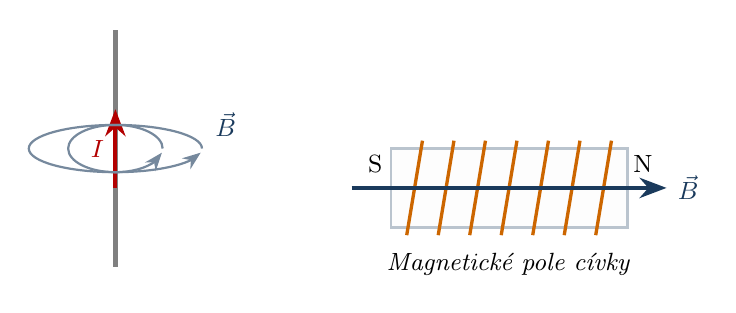
\begin{tikzpicture}[>=Stealth, font=\small, thick]
  % Vodič
  \draw[line width=2pt, gray] (0,-1) -- (0,2);
  \draw[->, red!70!black, line width=1.5pt] (0,0) -- (0,1) node[midway, left] {$I$};
  
  % Siločáry (elipsy)
  \foreach \r in {0.6, 1.1} {
    \draw[accent!60, ->] (\r,0.5) arc (0:350:{\r} and 0.3);
  }
  \node[accent] at (1.4, 0.8) {$\vec{B}$};
  
  % Cívka (solenoid)
  \begin{scope}[xshift=5cm]
    \draw[line width=1pt, accent!30, fill=lightgray!20] (-1.5,-0.5) rectangle (1.5,0.5);
    \foreach \x in {-1.2, -0.8, -0.4, 0, 0.4, 0.8, 1.2} {
      \draw[line width=1.2pt, orange!80!black] (\x-0.1,-0.6) -- (\x+0.1,0.6);
    }
    \draw[->, accent, line width=1.5pt] (-2,0) -- (2,0) node[right] {$\vec{B}$};
    \node at (1.7, 0.3) {N};
    \node at (-1.7, 0.3) {S};
    \node[below=0.7cm] at (0,0) {\textit{Magnetické pole cívky}};
  \end{scope}
\end{tikzpicture}
\end{center}

\begin{vzorcebox}
\[
\text{Vodič:} \quad B = \frac{\mu \cdot I}{2\pi \cdot r}
\qquad
\text{Cívka (uvnitř):} \quad B = \frac{\mu \cdot N \cdot I}{l}
\]
$\mu = \mu_0 \cdot \mu_r$ je \textbf{permeabilita} prostředí ($\mu_0 = 4\pi \cdot 10^{-7} \jednotka{N/A^2}$).
\end{vzorcebox}

% ================================================================
\subsection*{3. Vzájemné působení dvou vodičů}

Dva rovnoběžné vodiče na sebe působí magnetickou silou:
\begin{itemize}
  \item \textbf{Souhlasné proudy:} vodiče se \textbf{přitahují}.
  \item \textbf{Nesouhlasné proudy:} vodiče se \textbf{odpuzují}.
\end{itemize}

\begin{vzorcebox}
\[
F_m = \frac{\mu}{2\pi} \cdot \frac{I_1 \cdot I_2}{d} \cdot l
\]
\end{vzorcebox}

% ================================================================
\subsection*{4. Magnetické vlastnosti látek a hystereze}

Látky dělíme podle relativní permeability $\mu_r$:
\begin{enumerate}
  \item \textbf{Diamagnetické} ($\mu_r < 1$): mírně pole zeslabují (měď, zlato, voda).
  \item \textbf{Paramagnetické} ($\mu_r > 1$): mírně pole zesilují (hliník, platina, vzduch).
  \item \textbf{Feromagnetické} ($\mu_r \gg 1$): výrazně pole zesilují (železo, kobalt, nikl).
\end{enumerate}

U feromagnetik dochází k \textbf{magnetické nasycenosti} a projevuje se \textbf{magnetická hystereze} (zpoždění $B$ za $H$).

\begin{center}
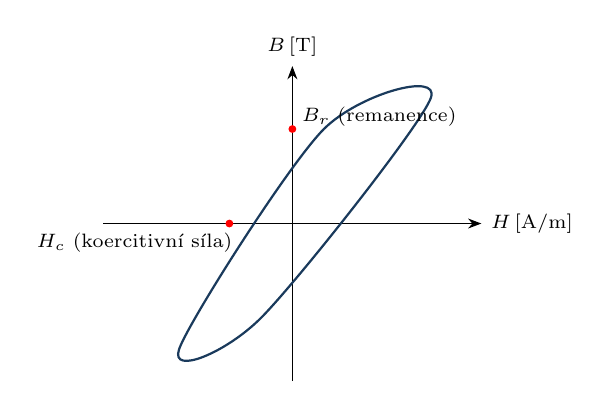
\begin{tikzpicture}[>=Stealth, font=\scriptsize, scale=0.8]
  % Osy
  \draw[->] (-3,0) -- (3,0) node[right] {$H \jednotka{A/m}$};
  \draw[->] (0,-2.5) -- (0,2.5) node[above] {$B \jednotka{T}$};
  
  % Hysterezní smyčka
  \draw[thick, accent] plot [smooth cycle] coordinates {(2.2,2) (0.5,1.5) (-1.8,-2) (-0.5,-1.5)};
  
  % Význačné body
  \node[circle, fill=red, inner sep=1pt] at (0,1.5) {};
  \node[right] at (0,1.7) {$B_r$ (remanence)};
  \node[circle, fill=red, inner sep=1pt] at (-1,0) {};
  \node[below left] at (-0.8,0) {$H_c$ (koercitivní síla)};
\end{tikzpicture}
\end{center}

% ================================================================
\subsection*{5. Elektromagnetická indukce}

Při změně magnetického pole v okolí vodiče/cívky vzniká (indukuje se) elektrické napětí.

\begin{durazbox}
\textbf{Faradayův zákon:} Indukované napětí je rovno časové změně magnetického indukčního toku.
\[
U_i = - N \cdot \frac{\Delta \Phi}{\Delta t}
\]
\textbf{Lenzovo zákon:} Indukovaný proud má takový směr, že svými účinky působí proti změně, která ho vyvolala (vyjádřeno znaménkem \textbf{minus}).
\end{durazbox}

\begin{center}
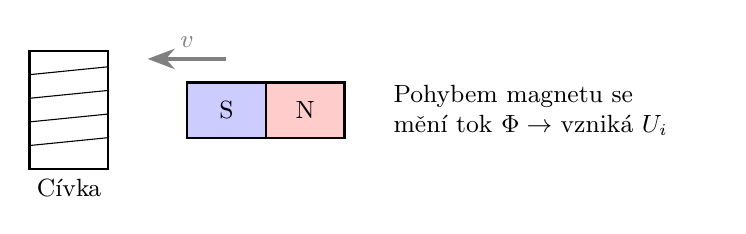
\begin{tikzpicture}[>=Stealth, font=\small]
  % Cívka
  \draw[thick] (0,0) rectangle (1,1.5);
  \foreach \y in {0.3, 0.6, 0.9, 1.2} \draw (0,\y) -- (1,\y+0.1);
  \node[below] at (0.5,0) {Cívka};
  
  % Magnet
  \draw[thick, fill=blue!20] (2,0.4) rectangle (3,1.1);
  \node at (2.5,0.75) {S};
  \draw[thick, fill=red!20] (3,0.4) rectangle (4,1.1);
  \node at (3.5,0.75) {N};
  
  % Pohyb
  \draw[->, line width=1.5pt, gray] (2.5,1.4) -- (1.5,1.4) node[midway, above] {$v$};
  \node[text width=4cm, right] at (4.5,0.75) {Pohybem magnetu se\\ mění tok $\Phi \rightarrow$ vzniká $U_i$};
\end{tikzpicture}
\end{center}

% ================================================================
\subsection*{6. Vlastní indukce a indukčnost}

Indukované napětí vzniká i ve vodiči samotném při změně proudu, který jím protéká. Schopnost cívky indukovat napětí popisuje \textbf{indukčnost $L$}.

\begin{vzorcebox}
\[
U_i = - L \cdot \frac{\Delta I}{\Delta t} \jednotka{V}
\qquad
L = \frac{N \cdot \Phi}{I} = \mu \cdot \frac{N^2 \cdot S}{l} \jednotka{H} \quad \text{(henry)}
\]
\end{vzorcebox}

\textbf{Energie magnetického pole cívky:}
\begin{vzorcebox}
\[
W_m = \frac{1}{2} \cdot L \cdot I^2 \jednotka{J}
\]
\end{vzorcebox}

% ================================================================
\subsection*{7. Shrnutí – přehled vzorců}

\begin{center}
\begin{tabularx}{0.97\linewidth}{@{} l l l @{}}
\toprule
\textbf{Veličina} & \textbf{Vzorec} & \textbf{Jednotka} \\
\midrule
Mag. indukční tok & $\Phi = B \cdot S \cdot \cos \alpha$ & Wb (weber) \\
Ampérova síla & $F_m = B \cdot I \cdot l \cdot \sin \alpha$ & N (newton) \\
Lorentzova síla & $F_L = Q \cdot v \cdot B \cdot \sin \alpha$ & N \\
Intenzita mag. pole & $H = I / (2\pi r) \text{ nebo } (N \cdot I) / l$ & A/m \\
Mag. indukce & $B = \mu \cdot H$ & T (tesla) \\
Indukované napětí & $U_i = - N \cdot \Delta \Phi / \Delta t$ & V (volt) \\
Indukčnost cívky & $L = \mu \cdot N^2 \cdot S / l$ & H (henry) \\
Energie mag. pole & $W_m = \frac{1}{2} L I^2$ & J (joule) \\
\bottomrule
\end{tabularx}
\end{center}

\end{vysvetlenibox}

\end{document}